\chapter{Diseño de un chatbot de ayuda a la terapia a la reminiscencia}
\label{cap:ChatBot final}
Este capítulo tiene como objetivo presentar la solución final desarrollada a partir de la problemática presentada en el capítulo \ref{sec:objetivos}. Para ello, se describirá en profundidad cada uno de los componentes básicos de la arquitectura del sistema, y se presentara esta en sí misma. Por otro lado, se explicará tanto el proceso de puesta en marcha como las herramientas necesarias para ese mismo objetivo. 

Con el objetivo de permitir la opción de estudiar los componentes de forma práctica, es decir, usando el prototipo, este capítulo comenzará por la explicación de la puesta en marcha. A continuación, se dará una idea global de la arquitectura del sistema y finalmente se irá explorando en cada sección, cada uno de los módulos que la componen. 
\section{Herramientas y puesta en marcha}
Para la puesta en marcha el primer paso es obtener la \textit{API Key} para lo que es necesario el uso de una VPN.
\subsection{VPN}
Debido a las restricciones geográficas actuales de la API de Gemini para poder usarla es necesario el uso de una VPN. En concreto y para el desarrollo de este proyecto la conexión a la VPN se ha realizado mediante la herramienta \textit{hide.me VPN}. Esta herramienta crea un túnel seguro utilizando poderosos protocolos VPN, oculta nuestra IP real con una suya y cifra todo el tráfico de internet que pasa por este túnel para que podamos navegar libremente. Además, \textit{hide.me} está certificada como una VPN cero registros. Esto significa que no se almacena información de ningún tipo. El uso de la VPN es necesario tanto para obtener la \textit{API Key} como para el uso de la misma. Los países en los que se encuentra disponible gemini se pueden consultar en la web \href{https://ai.google.dev/gemini-api/docs/available-regions?hl=es-419} de la api de gemini. 

\subsection{Instalación de la API de Gemini}

Para comenzar a utilizar la API de Gemini con Python, es necesario seguir estos pasos para instalar el SDK y configurar tu clave de API.

En primer lugar, instalamos el SDK (Software Development Kit). La API de Gemini está contenida en el paquete \texttt{google-generativeai} en PyPI, por lo que el primer paso sera instalar esa dependencia.

\begin{lstlisting}[language=Python]
	!pip install -U google-generativeai
\end{lstlisting}

Para utilizar la API de Gemini, se necesita una clave de API obtenida del \href{https://aistudio.google.com/app/apikey} Google AI Studio. Una vez que tengas tu clave, puedes configurarla para que el SDK la utilice:

\begin{lstlisting}[language=Python]
	import google.generativeai as genai
	from google.colab import userdata
	
	GOOGLE_API_KEY = userdata.get('GOOGLE_API_KEY')
	genai.configure(api_key=GOOGLE_API_KEY)
\end{lstlisting}


Siguiendo con la arquitectura del sistema bastaría con modificar en el archivo \textit{config.py} el valor de la \textit{API KEY}.

\subsection{Puesta en marcha} 
Una vez hechas todas las configuraciones necesarias explicadas en las secciones anteriores, para poder usar el chatbot sería necesario poner en ejecución el módulo $mibot.py$ y enviar el comando $\backslash start$ al usuario $\makeatletter @ mavice07\_bot$. Es importante recordar, que para que el análisis de la información y el flujo de la conversación se desarrollen correctamente, hay que esar conectado a una VPN de una de las localizaciones en las que se encuentra disponible la API de gemini, y que como ya se ha comentado con anterioridad, se pueden consultar en \href{https://ai.google.dev/gemini-api/docs/available-regions?hl=es-419} la web de Gemini.
\section{Arquitectura del sistema}
Con todo lo implementado, el sistema se puede representar como se ve en la figura \ref{fig:arquitectura}. 

\begin{figure}[h]
	\centering
	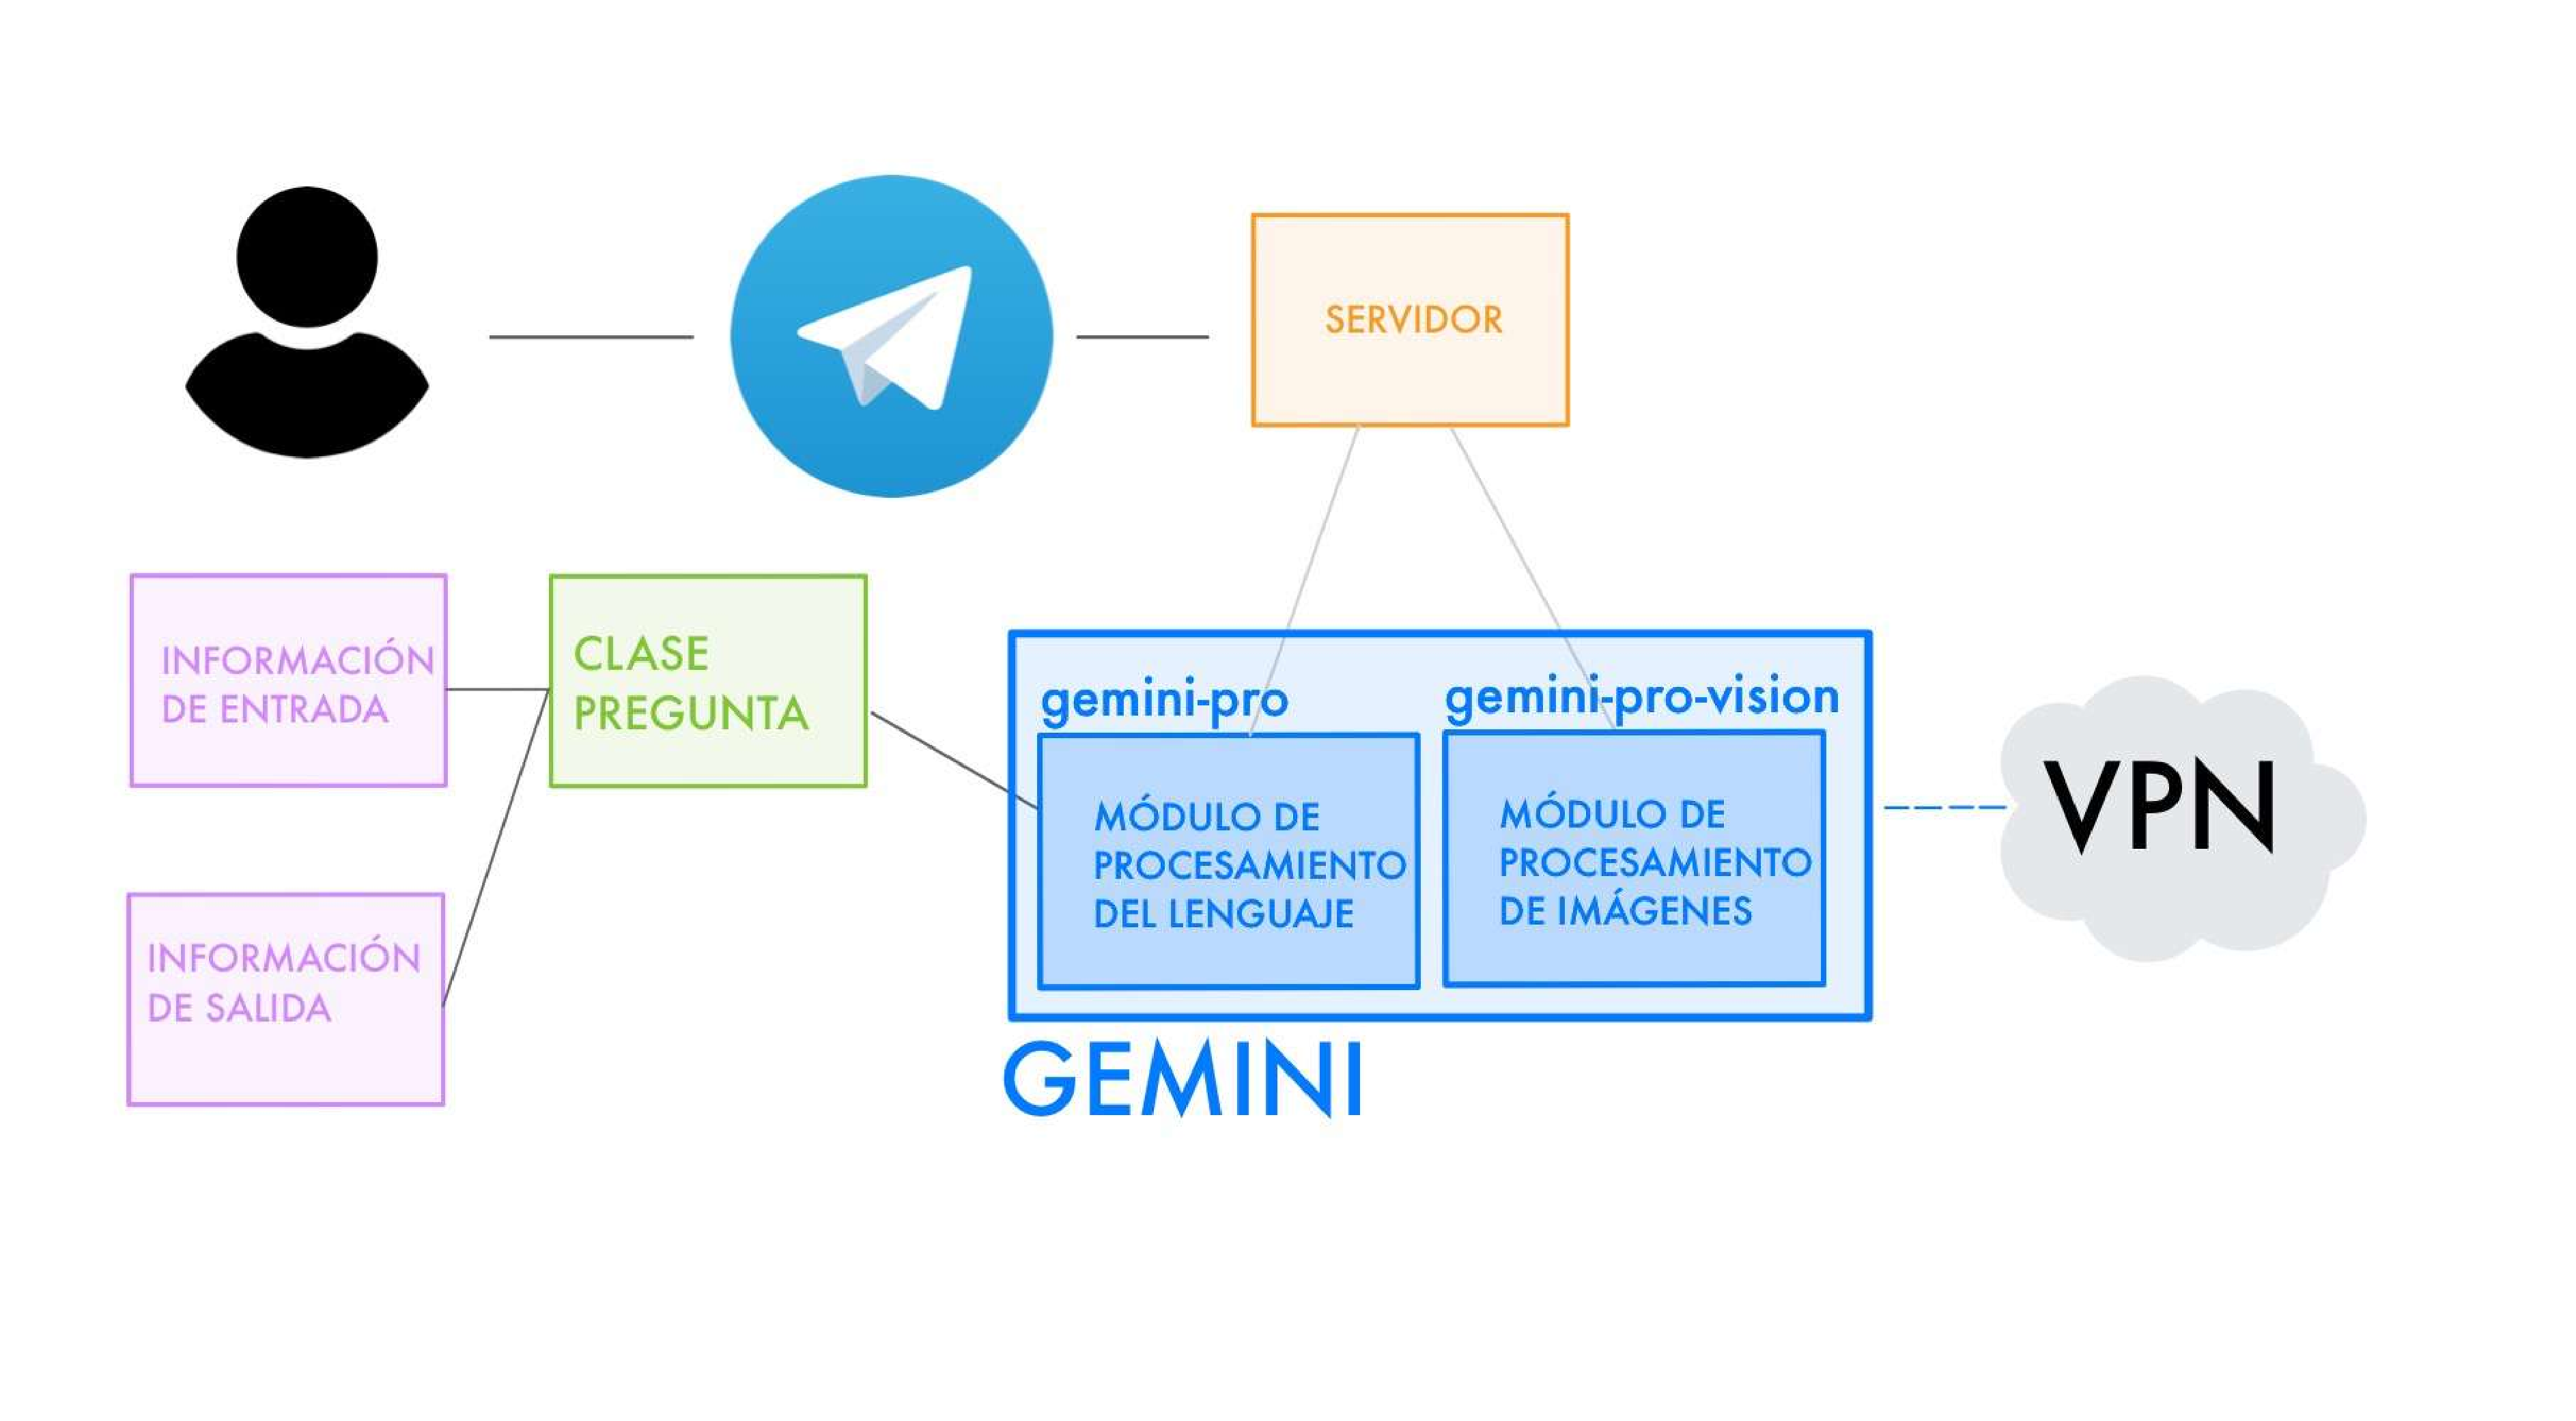
\includegraphics[width=1\textwidth]{Imagenes/arquitectura}
	\caption{Arquitectura del sistema}
	\label{fig:arquitectura}
\end{figure}

\subsection{Servidor}

El módulo servidor se encarga de manejar el flujo de los mensajes del chatbot. Recibe los mensajes entrantes desde la plataforma de Telegram y coordinar su procesamiento posterior. Este módulo actúa como el punto de entrada centralizado del sistema, y ha de mantenerse en ejecución durante todo el tiempo en el que se quiera usar el chatbot.

La lógica del módulo para manejar los mensajes sigue lo explicado en la sección \ref{sec:Telegram}, utilizando distintos manejadores según el tipo de mensaje.  Esta capacidad de coordinación del módulo servidor asegura una distribución eficiente de los mensajes entrantes optimizando así la velocidad de respuesta y la efectividad de las interacciones con los usuarios.

El módulo servidor sirve como el núcleo activo del chatbot, recibiendo mensajes desde Telegram y dirigiéndolos de manera inteligente hacia los componentes adecuados del sistema para su procesamiento y respuesta. Su función es fundamental para mantener el flujo de comunicación entre los usuarios y el chatbot, facilitando una experiencia de usuario fluida y receptiva.

\subsection{Procesamiento}
El módulo del procesamiento de la información es el que usa Gemini, y que por tanto requiere estar conectado a una VPN. En función del tipo de mensaje de entrada, imagen o texto, el servidor enviará la información al módulo de procesamiento del lenguaje o al módulo del procesamiento de imagenes.
\subsubsection{Módulo de procesado de la información}
Este módulo reune la mayoría de la funcionalidad del chatbot. En concreto se encarga de las siguientes tareas: 
\begin{itemize}
	\item Análisis de las respuestas 
	\item Identificación de la información faltante
	\item Flujo de las preguntas
	\item Generación de los json con la información
	\item Generación de preguntas adicionales 
	 \item Generación de la historia de vida final
\end{itemize}
Todas estas funcionalidades ya se han explicado con más detalle en el capítulo \ref{cap:Desarrollo de prototipos}. La funcionalidad adicional que aparece es generación de la historia de ida final. Esta funcionalidad no es un objetivo en sí del sistema, si no que se crea, a raíz de toda la información obtenida y utilizando el Gemini para dar un feedback final al usuario, a modo de recopilación de la información.
\subsubsection{Módulo de procesado de imágenes}
Este módulo se encarga de cargar las imagenes que se han enviado a Telegram. Por las características del modelo y la arquitectura del sistema, cuando la imagen se envía a través de Telegram el manejador descarga la imagen y la almacena con un determinado nombre, que pasa como atributo al módulo de procesado de imágenes. Una vez hecha la llamada al procesado de imágenes el modelo carga la imagen, la analiza y genera una respuesta a partir de la propia imagen y de un prompt adecuado que en concreto, lo que le pide es que la describa de forma que haga al usuario alguna pregunta. De esta forma, se busca que las imagenes sirvan para obtener información adicional que con solo texto quizas el usuario no hubiera recordado. 

\subsection{Almacenamiento y manejo de la información}

El manejo de la información se lleva a cabo a través de ficheros. Cuando el servidor recibe el comando $\backslash start$ carga y crea las preguntas del fichero \textit{preguntas.txt}. Una vez llevada a cabo toda la conversación con el usuario, la información obtenida y la información generada se guardan en el fichero de salida \textit{información.txt}

\section{Interfaz e interacción con el usuario}
A pesar de que se podría usar a través de su versión por consola, el chatbot esta pensando para ser usado a través de Telegram. Gracias a esto se puede usar desde tantos dispositivos como se puede usar Telegram, entre los que destacaríamos los dispositivos móviles y los ordenadores.

Para poner en marcha la versión por ordenador, es necesario la aplicación de Telegram, ya sea la versión web o la versión local. De igual forma la versión en móvil u tablet requiere la aplicación de Telegram. Una vez con la aplicación correctamente instalada y abierta, hay que buscar al usuario $\makeatletter @ mavice07\_bot$ y enviado el comando  $\backslash start$, recibiremos el mensaje de bienvenida y comenzará la conversación. Ejemplo de esto en la versión de ordenador y móvil se pueden ver respectivamente en las figuras \ref{fig:bienvenidaOrdenador} y \ref{fig:bienvenidaMovil}.

\begin{figure}[h]
	\centering
	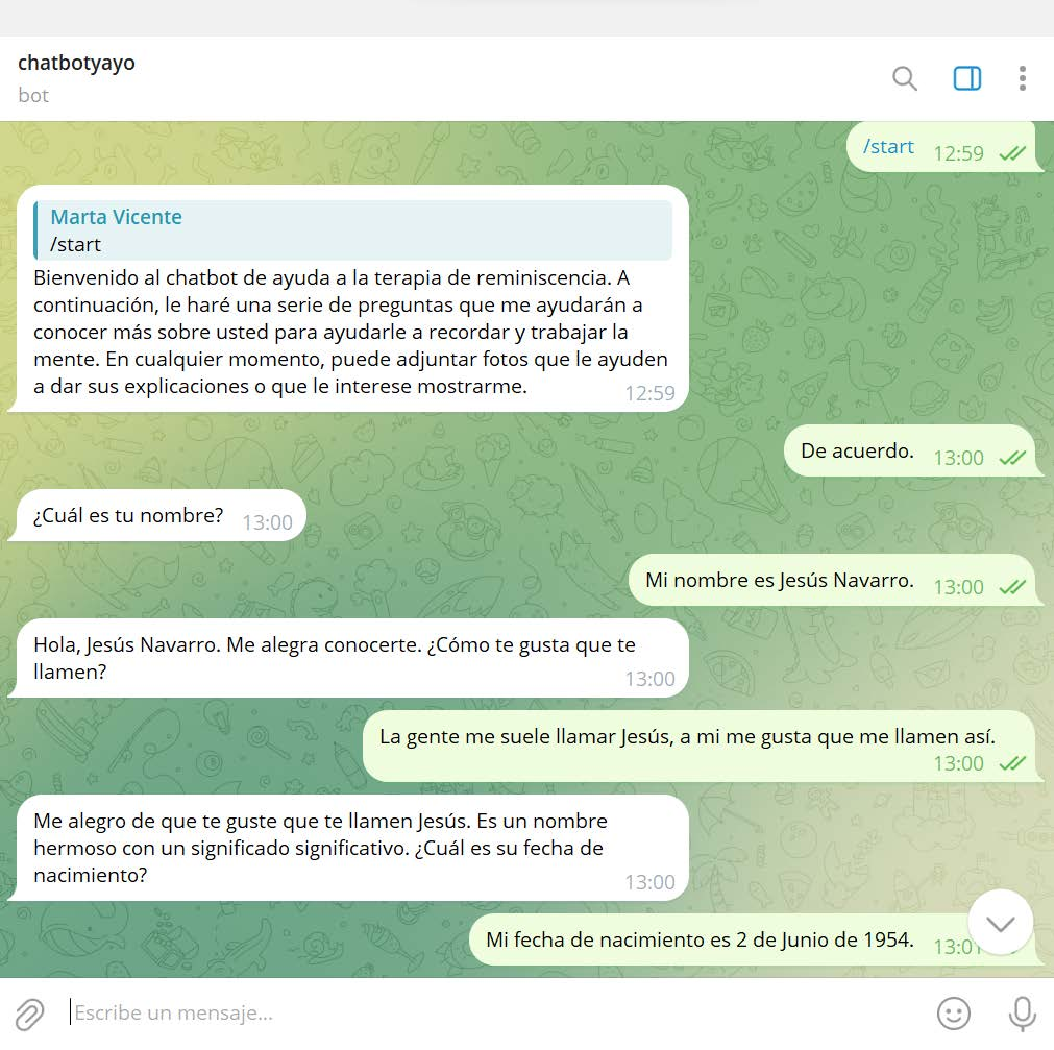
\includegraphics[width=0.6\textwidth]{Imagenes/bienvenidaOrdenador}
	\caption{Ejemplo de bienvenida y primeras interacciones con la versión en ordenador}
	\label{fig:bienvenidaOrdenador}
\end{figure}

\begin{figure}[h]
	\centering
	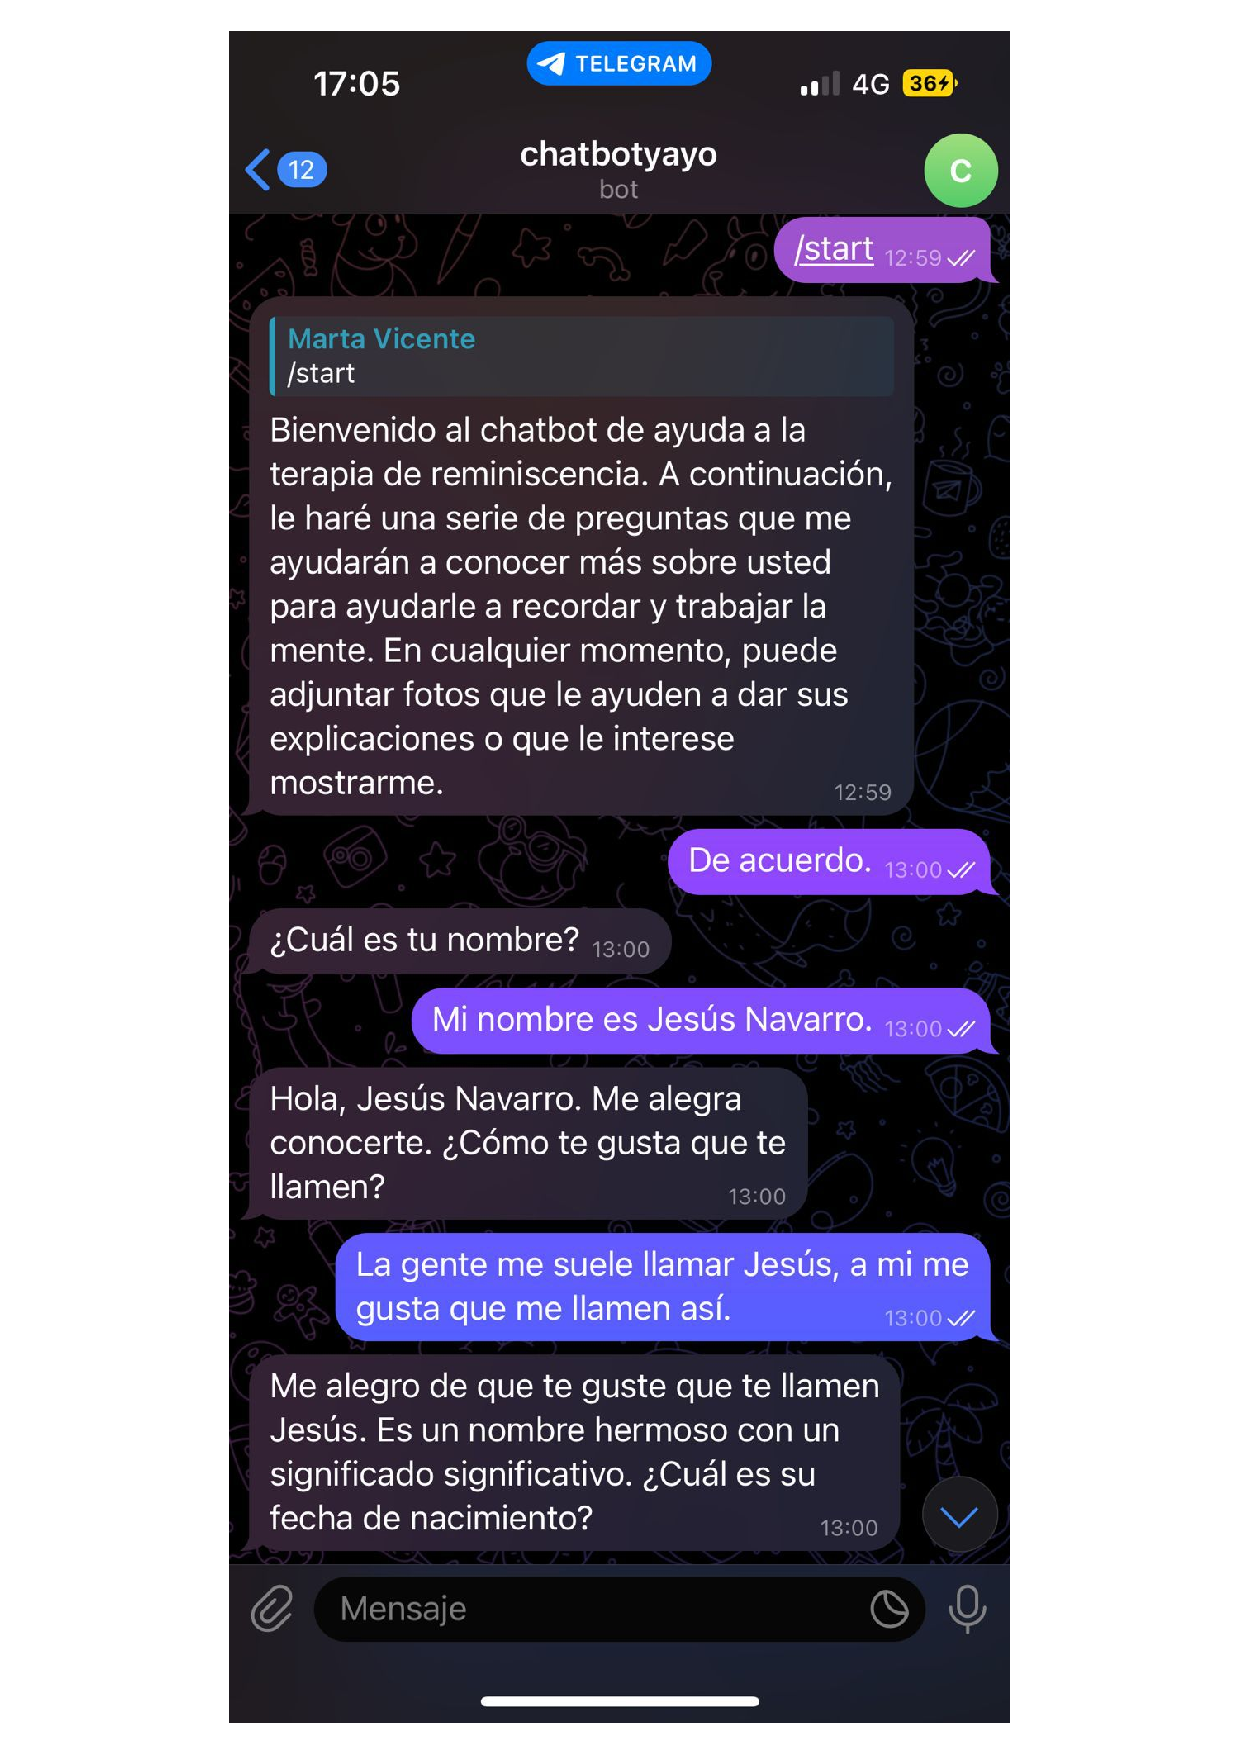
\includegraphics[width=0.6\textwidth]{Imagenes/bienvenidaMovil}
	\caption{Ejemplo de bienvenida y primeras interacciones con la versión en móvil}
	\label{fig:bienvenidaMovil}
\end{figure}



